% Optional appendix, submitted as a SEPARATE PDF (the 2027 call allows one, with no page limit).
% Reviewers may choose not to read it, so nothing load-bearing goes here: only the full tables,
% the per-seed numbers, the scorer calibration, the controls and the exact commands. Every section
% here is referenced from the main text by the same letter.
\documentclass[10pt,letterpaper]{article}
\usepackage[margin=1in]{geometry}
\usepackage[T1]{fontenc}\usepackage[utf8]{inputenc}\usepackage{times}
\usepackage{graphicx}\usepackage{booktabs}\usepackage{amsmath}\usepackage{siunitx}
\usepackage{multirow}
\usepackage{xcolor}\usepackage[hidelinks]{hyperref}\usepackage{longtable}
\usepackage[font=small,labelfont=bf]{caption}
\graphicspath{{figures/}}
\newcommand{\TODO}[1]{\textcolor{red}{[TODO: #1]}}
\newcommand{\NUM}[1]{\textcolor{blue}{#1}}
\newcommand{\nt}{\,nt}
\newcommand{\bits}{bits/nt}
\newcommand{\excess}{\textit{excess}}
\newcommand{\kmer}[1]{#1-mer}
\renewcommand{\thesection}{A\arabic{section}}
\title{\textbf{Appendix:} Tokenisation and Training Objective Determine Memorisation in Genomic
Language Models}
\author{}\date{}
\begin{document}\maketitle\vspace{-3em}

\section{Scorer calibration}
\TODO{A1. The two masked-model scorers (pseudo-log-likelihood and prefix-conditioned) and why both
are kept: on synthetic DNA the PLL scorer sits at 2.0006 bits/nt while the prefix scorer drifts to
2.04--2.05 for models trained at a 15\% mask rate. Table of the chance level measured for every
(tokeniser, objective) cell, which is the sanity check that makes every later number readable.}

\section{Per-seed tables}
\TODO{A2. Everything the main text reports as a seed mean, per seed: controlled grid, DNABERT family
on four datasets, DNABERT-2 and HyenaDNA, human chromosome 22 across the four canary-split draws.}

\section{Capacity and parametrisation controls}
Non-embedding parameters are identical (12.61M) in every controlled cell, so only the embedding
table changes with the vocabulary. The three controls below, and the spaced $k$-mer tokenisers that
hold the token-sequence length fixed while changing the vocabulary, are what the main text's
robustness claim rests on.

\paragraph{What the tokeniser effect is robust to, and what it is sensitive to.}
Every cell has the same 12.61M non-embedding parameters, so only the embedding table changes with the
vocabulary, and three controls probe whether the effect is really about the table. It is not about
its size: factorising the embedding to rank~512 is a pure reparametrisation --- $E' = EW^{\!\top}$
with the same tie between input and output, hence the same function class --- yet it moves the
\kmer{6} from \NUM{0.61} to \NUM{1.44}~\bits{} at matched held-out loss, roughly the \kmer{3} level,
and ranks 27 to 256 behave the same, so there is no dose--response in embedding parameters. It is
also not a learning-rate artefact of the embedding rows: lowering only the embedding learning rate
makes the \kmer{6} memorise \emph{more} per unit of overfitting, the opposite of that hypothesis.
What survives all of it is the character-to-\kmer{3} step, which is parameter-matched to begin with
and unchanged by every variant. \textbf{We therefore report the large-vocabulary excess as a range
rather than a constant}: for the identical function class it runs from near zero (factorised
embedding) to large (low embedding learning rate), which means memorisation here is a property of
the training dynamics and not only of the architecture --- the same conclusion the paper draws about
architecture labels, applied to our own grid.

\paragraph{Above capacity the effect becomes qualitative.}
Pretrained genomic models are trained far above their capacity, so the interesting regime is the one
where the corpus cannot be stored. At $20\times$ data (100{,}000 windows, about 57.6M bits against a
capacity estimate of roughly 45M bits for 12.6M parameters \cite{morris2025capacity}) the three
tokenisers separate absolutely rather than quantitatively, and it replicates across seeds: the
character model memorises \emph{nothing} --- every canary at chance, including those seen
$16 \times 30 = 480$ times --- the \kmer{3} is at chance, and the \kmer{6} recognises every member
canary including those seen once per epoch and extracts every $16\times$ canary verbatim from
round~8. One caveat we cannot yet separate: $20\times$ data at a fixed round count is also
$20\times$ more updates between canary exposures, so capacity and interference are confounded here
(Appendix~A7). The ordering is the same as at $1\times$ data; only its sharpness changes.
\TODO{add the per-rank table (27, 64, 128, 256, 512), the feed-forward width control and the spaced
$k$-mer numbers; they are in \texttt{outputs/cap\_*/gate1\_report\_final.md} and
\texttt{outputs/len\_sp/}.}

\section{Position encoding and canary placement}

\begin{figure}[t]
\centering
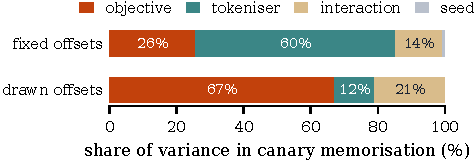
\includegraphics[width=0.6\textwidth]{figures/F3_variance.pdf}
\caption{share of the variance in canary memorisation, by factor, over the controlled
grid (24 runs). With independently drawn canary offsets the objective dominates; with every copy at
the same offset the tokeniser appears to, because a model with learned absolute positions can score
a record from its position. Restricted to the three tokenisers both arms share, the drawn-offset
shares are \NUM{57.7}, \NUM{15.4}, \NUM{26.9} and \NUM{0.0}\,\%. \label{fig:variance}
\end{figure}

\paragraph{The same decomposition, run before we fixed the placement, says the opposite.}
With every canary copy at the same offset inside its host window, the identical analysis attributes
\NUM{59.5\%} to the tokeniser and \NUM{25.7\%} to the objective: the two leading factors trade
places. The reason is that a model with learned absolute positions can score a canary from its
position alone, and coarse tokenisers align to that offset, so fixed placement manufactures a
tokeniser effect (Appendix~A4). This is a finding about how to run the measurement rather than about
the models, and it is why every number in this paper uses independently drawn offsets. We report both
decompositions because the difference between them is larger than most effects anyone would publish
from either one.
\TODO{add the RoPE comparison and the per-offset table from \texttt{outputs/off1} and
\texttt{outputs/rope\_rand}.}

\section{Real canary construction}
\TODO{A5. The 1000 Genomes filter (AC/AN $\le$ 0.001, at most 5 carriers), the 400 segments, the 366
carriers, the allele-frequency distribution, and the two methodological points: the ranking pool and
the fresh host must both be real, and the INFO AF field is rounded to two decimals so the frequency
must come from AC/AN.}

\section{Downstream probe}

\begin{table}[t]
\centering
\caption{Downstream score and leakage move independently. Fine-tuned Matthews correlation on the
task's full test split, three seeds, beside the $16\times$ canary of the \emph{same} checkpoint; the
DNABERT \kmer{6} shown as the example, with the across-model movement in the last row.
\TODO{decide whether the per-model panels go to the appendix; they are all in
\texttt{utility\_downstream.md}.}}
\label{tab:downstream}
\begin{tabular}{lcccccc}
\toprule
round & held-out loss & recognised & extracted & promoter & splice & histone H3 \\
\midrule
1  & 2.027 & 0\%   & 0\%   & 0.844 & ---   & 0.709 \\
3  & 1.934 & 8\%   & 0\%   & 0.860 & 0.782 & 0.727 \\
8  & 1.922 & 30\%  & 0\%   & 0.857 & 0.782 & 0.717 \\
15 & 1.916 & 88\%  & 0\%   & 0.855 & 0.803 & 0.733 \\
30 & 1.940 & 100\% & 44\%  & 0.860 & 0.801 & 0.728 \\
50 & 2.027 & 100\% & 95\%  & 0.855 & 0.801 & 0.728 \\
\midrule
\multicolumn{4}{l}{movement over rounds 1--50, all six models} & $\le$0.027 & $\le$0.147 & $\le$0.028 \\
\bottomrule
\end{tabular}
\end{table}

\paragraph{Probe validity.}
Our fine-tuning is a scaled-down version of the published recipe (two rounds over up to 20{,}000
labelled sequences, where the published recipe uses three over the full split), so our absolute
scores are below the published ones and only the movement within a column is ours to interpret. On
five tasks they land in the same range --- promoter \NUM{0.79}--\NUM{0.86}, core promoter
\NUM{0.59}--\NUM{0.66}, TF binding \NUM{0.61}--\NUM{0.68}, splice \NUM{0.60}--\NUM{0.80}, H3
\NUM{0.68}--\NUM{0.74}. On yeast H3K4me3 the head reaches only \NUM{0.22}--\NUM{0.30}, far enough
below the published figure that we treat that row as a weak probe rather than a reproduction
(Appendix~A6). \TODO{quote the published GUE MCCs for these six tasks from
\cite{zhou2024dnabert2} once checked against the paper's own table, and say which of the five are
within 0.05 of it.} Four of the \NUM{252} (model, round, task) fine-tuning runs collapsed to a
degenerate head --- MCC \NUM{0.000}, \NUM{0.000}, \NUM{0.086} and \NUM{0.000} where the same model
and task score at or near the median at every other round, all four of them in DNABERT-2 or at
round~0 or~1 --- and they are excluded from the movement statistics above and listed in the
appendix. That is the only exclusion anywhere in this paper.
\TODO{add the per-model, per-round, per-task MCC panels from
\texttt{outputs/dnabert\_gue\_ds/utility\_downstream.md}, and list the four degenerate fine-tuning
runs (DNABERT-2 splice r0, DNABERT-2 H3K4me3 r0 and r1, DNABERT 6-mer splice r1).}

\section{Exact commands}
\TODO{A7. One command per table and figure in the main text, from the queue scripts in
\texttt{pilot2/}.}

\section{Edge-conditioned extraction audit}

\paragraph{Asked in its own idiom, the masked model still returns nothing.}
A masked model does not have to be read left to right, and prefix-only probing is the weak way to
ask it: on diffusion language models, edge-conditioned masks recover up to three times more verbatim
sequences than prefix-conditioned ones \cite{wang2026infilling}. Our extraction ruler is
prefix-conditioned, which is the right default for comparing two objectives on equal terms but the
wrong one for clearing a masked model, so we re-ran every masked cell with the sequence after the
record left visible and the 48 masked nucleotides decoded in confidence order --- the model's own
idiom and the stronger attack. Across all five datasets, every tokeniser, both mask rates, two to
three seeds and all three repetition tiers (120 cells, 20 canaries each), edge-conditioned
extraction recovers \textbf{no} record: \NUM{0\%} under both protocols, with \NUM{34.9} wrong
nucleotides out of 48 under the prefix protocol and \NUM{35.2} under infilling, against
\NUM{35.0}--\NUM{35.6} for non-members. The member cells are at the non-member level under the
protocol designed to break them, including the leakiest masked cells in the paper (the human
\kmer{6} at $50\%$ masking, \excess{} \NUM{0.29}), which is the strongest form in which we can state
this recommendation.
\TODO{add the full 120-cell table from \texttt{outputs/human\_mlm/infill\_audit.md}.}

\section{Natural duplicates, full table}
\TODO{A10. The complete table from \texttt{outputs/human\_big/human\_big2\_natural.md}: four
tokenisers x five multiplicities x trained and held-out, with bits/nt and rank-1 beside verbatim
extraction, and the corpus census (1{,}006{,}401 blocks once, 2{,}235 twice, 1{,}245 three or four
times, 717 five to eight, 68 nine or more).}

\section{Re-drawing the member/non-member canary split}

\paragraph{Why the canary split needs four draws, and why the obvious correction is wrong.}
Which canaries are members and which are matched controls is fixed by one data seed, so within an arm
it is the same split for every model and every model seed. With real haplotype canaries the two
groups of 50 segments differ by chance, and before any fine-tuning the released checkpoints already
read the member group as easier --- up to \NUM{0.9}~\bits{} on a single draw, against
$\pm$\NUM{0.09} for HyenaDNA, the one causal-pretrained model in the panel. It is tempting to treat
that as a fixed offset and subtract it. Re-drawing the split four times shows that this is the wrong
correction: the offset is gone after a single epoch of fine-tuning (\excess{} at round~1 is
\NUM{0.00}$\pm$\NUM{0.05} for every model on every draw, whatever the round-0 reading was), a
regression of each draw's round-50 \excess{} on its own round-0 offset has slope
\NUM{0.05}--\NUM{0.19}, and subtracting the offset in full accordingly inflates the across-draw
spread from \NUM{0.04}--\NUM{0.11} to \NUM{0.15}--\NUM{0.39}. We therefore report the uncorrected
statistic, quote the across-draw spread as its error bar, and treat the round-0 reading as a
diagnostic: it measures the instability of a pretrained model's prior over two sets of real
haplotypes, not a property of the canaries. On the three random-canary datasets the offset is
negligible ($\le$\NUM{0.15}), as it must be where the two groups are exchangeable by construction.
\TODO{add the per-draw table (data seeds 1234, 2345, 3456, 4567): round-0 offset, round-50 excess
raw and baseline-corrected, and the regression of the second on the first.}

\end{document}
